\chapter{SPECTRE attacks}
	\index{Spectre}In questo capitolo verrà presentato \emph{SPECTRE}\cite{kocher2018spectre}, un tipo di attacco molto recente che sfrutta una vulnerabilità presente nella maggior parte dei processori moderni (Intel, AMD e ARM) e per il quale, al momento, non esistono contromisure.
	
	La vulnerabilità che viene sfruttata da questo tipo di attacco è la cosiddetta \emph{esecuzione speculativa}.
	
	\section{Esecuzione speculativa}
		\index{Esecuzione speculativa}L'esecuzione speculativa è una tecnica utilizzata dai processori per migliorare le prestazioni che consiste nel cercare di "indovinare" il risultato di un branch per eseguire preventivamente alcune istruzioni.
		
		Supponiamo ad esempio che l'esecuzione del programma dipenda da un controllo su di un valore non presente in cache che quindi deve essere recuperato dalla memoria principale. Questo può portare ad un attesa di svariate centinaia di cicli clock prima che questo valore sia disponibile. Invece di aspettare tutto questo tempo inutilmente, il processore cerca di indovinare il risultato del controllo, salva lo stato attuale dei suoi registri, e procede ad eseguire speculativamente il ramo del branch che ritiene più plausibile (supponiamo il ramo then). Quando poi arriverà il valore effettivo dalla memoria, il controllo verrà effettivamente effettuato. Se il risultato è quello aspettato (true nel nostro caso), si procede con la computazione e saranno stati risparmiati tutti quei cicli di clock che sarebbero stati persi nell'attesa. Se la scelta si rivela sbagliata (false), il processore scarta tutti i risultati dell'esecuzione speculativa, si riporta allo stato che si era salvato precedentemente ed esegue l'altro ramo del branch (else).
		
		Questa ottimizzazione sembra perfetta in quanto in caso di successo, si risparmiano molti cicli di clock mentre in caso di insuccesso il risultato è paragonabile a quello che avremmo ottenuto aspettando il dato senza eseguire alcuna istruzione.
		
		Il responsabile di questa scelta è una piccola unità all'interno del processore chiamata \ac{BP}.
		
		\subsection{Branch predictor}
			\index{Branch Predictor}Esistono svariati tipi di branch predictor; andiamo a vedere come funziona uno dei più semplici, il \emph{one-level branch predictor} a 2 bit.
			
			\begin{figure}
				\begin{center}
					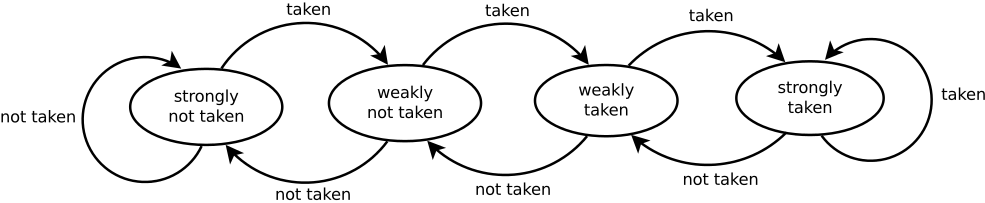
\includegraphics[scale=.35]{bp2bit}
					\caption{Automa di predizione di un one-level branch predictor a 2 bit}
					\label{fig:bp2bits}
				\end{center}
			\end{figure}
		
			Come da schema in \cref{fig:bp2bits} un one-level branch predictor può essere descritto con un semplice automa a 4 stati.
			
			\begin{enumerate}
				\item \emph{Strongly not taken:} in questo stato il \ac{BP} sceglierà il ramo else del branch. In caso di risultato effettivamente negativo resterà in questo stato altrimenti passerà allo stato 2.
				\item \emph{Weakly not taken:} in questo stato il \ac{BP} ha già osservato una esecuzione then ma la sua scelta resterà ancora il ramo else. Se il controllo si rivelerà false, il \ac{BP} tornerà allo stato 1 ma se si rivelerà true andrà allo stato 3 dal quale inizierà a scegliere il ramo then.
				\item \emph{Weakly taken:} come detto in precedenza, in questo stato il \ac{BP} inizierà ad eseguire speculativamente il ramo then. Se da questo stato si ottiene un false, torneremo allo stato 2, altrimenti passeremo al 4.
				\item \emph{Strongly taken:} questo stato è il duale dello stato 1. In questa situazione il \ac{BP} eseguirà il ramo then rimanendo in questo stato se otterrà un true e tornando allo stato 3 se otterrà un false (continuando comunque ad eseguire il ramo then).
			\end{enumerate}
		
			In questo caso vediamo come l'esecuzione consecutiva di al più due rami then ci porta sicuramente in uno stato in cui il ramo scelto dal \ac{BP} sarà sicuramente quello then. Questa informazione sarà molto utile quando dovremo effettuare un training sul \ac{BP} per convincerlo ad eseguire il ramo then quando si troverà davanti ad un certo branch.
			
	\section{L'attacco}
		L'attacco SPECTRE induce la vittima ad eseguire speculativamente operazioni che non dovrebbero essere eseguite durante l'esecuzione corretta del programma. Da tali operazioni si otterranno poi le informazioni ricercate tramite un side-channel temporale.
		
		L'attacco si può scomporre in tre fasi:
		\begin{enumerate}
			\item \emph{Fase di setup:} in questa fase l'attaccante esegue delle operazioni che convincono il \ac{BP} ad eseguire il ramo then in caso si rendesse necessaria una esecuzione speculativa. In questa fase si cerca anche di costruire tale necessità ad esempio eseguendo letture di memoria che rimuovono dalla cache un valore che sarà poi necessario successivamente. Come ultima cosa l'attaccante può iniziare a preparare la porzione di cache dalla quale estrarrà il valore che vuole carpire alla vittima (ad esempio eseguendo il flush o l'evict di una line o di un set).
			\item \emph{Esecuzione speculativa:} in questa fase il processore esegue speculativamente delle istruzioni che esporrano informazioni confidenziali della vittima recuperabili tramite un side-channel. Tale esecuzione può esporre dati sensibili attraverso una vasta gamma di side-channels ma nell'articolo gli autori si concentrano sulla possibilità di recuperare un valore che risiede ad un indirizzo preciso nella memoria della vittima attraverso un attacco di tipo Flush+Reload o Evict+Reload.
			\item \emph{Recupero del dato:} come ultimo passo, viene montato l'attacco alla cache (Flush+Reload o Evict+Reload). Il recupero del dato si ottiene andando a misurare il tempo necessario alla lettura dall'indirizzo di memoria presente nella line sotto attacco.
		\end{enumerate}
			